\section{Resultados}
En los sistemas biológicos las partículas se encuentran aleatoriamente orientadas, por lo que es conveniente calcular las secciones transversales promedio $\langle C_{abs}\rangle$ y $\langle C_{sca}\rangle$, que consideran que las partículas se iluminan con ondas electromagnéticas con polarización a lo largo de sus tres ejes principales de forma homogénea, \footnote{Considerando que las partículas no sean ópticamente activas.} éstas están dadas por \cite{Bohren}:
\begin{align*}
	\langle C_{abs}\rangle &= \frac{k}{3} \text{Im}\{\alpha^{(1)}+\alpha^{(2)}+\alpha^{(3)}\},\\
	\langle C_{sca}\rangle &= \frac{k^4}{3(6\pi)} \left(\alpha^{(1)}+\alpha^{(2)}+\alpha^{(3)}\right)^2.
\end{align*}
Por la forma discoide cóncava que presentan los eritrocitos, en este trabajo, como primera aproximación, se realizaron los cálculos para elipsoides oblatos, con lo que se satisface que $C_{ext}^{(1)}=C_{ext}^{(2)}$, que corresponden a las secciones transversales producidas al aplicar un campo  polarizado en las direcciones $\hat{e}_x$ y $\hat{e}_y$, respectivamente. \\

Las propiedades de esparcimiento pueden ser descritas mediante la función dieléctrica $\epsilon(\omega)$ \cite{Plasmonics}, que puede ser determinada experimentalmente al medir el índice de refracción complejo de un medio $\tilde{n}(\omega)=n(\omega)+ik(\omega)$ definido como $n(\omega)=\sqrt{\epsilon(\omega)}$, que deviene en \cite{Plasmonics}
\begin{align}
	\text{Re}[\epsilon(\omega)]&=n^2-\kappa^2,\\
	\text{Im}[\epsilon(\omega)]&=2n\kappa,
\end{align}
con $\kappa$ el coeficiente de extinción, que determina la absorción de las ondas electromagnéticas al propagarse a través del medio. Para describir la función dieléctrica, se propone utilizar el modelo de Drude, que representa el movimiento de los electrones libres de un material ante la presencia de un campo eléctrico oscilante \cite{Plasmonics}
\begin{equation}
	\epsilon(\omega)=1-\frac{\omega_p^2}{\omega^2+i\gamma\omega},
\end{equation}
donde $\omega_p$ y $\gamma$ son cantidades propias del material, que corresponden a la frecuencia de plasma y la constante fenomenológica de amortiguamiento, respectivamente. Como este modelo asume que los electrones se mueven libremente, su validez depende del rango de frecuencias en el que se presentan transiciones interbanda. Este modelo, debido a su única dependencia con la frecuencia, permite un mayor control sobre la respuesta óptica, por lo que se emplea como  \\

Para determinar las contribuciones de las secciones transversales en partículas elipsoidales oblatas en el régimen cuasiestático, en la Fig. \ref{Contribuciones} se grafican las secciones transversales extinción, esparcimiento y absorción promedio $\langle C_{ext}\rangle$, $\langle C_{sca}\rangle$ y $\langle C_{abs}\rangle$, respectivamente, en escala logarítmica, como función de la longitud de
onda $\lambda$ y la energía $\hbar\omega$ para una partícula elipsoidal oblata descrita por una función dieléctrica tipo Drude con parámetros $\hbar\omega_p=13.142\text{ eV}$ y $\hbar\gamma=0.197\text{ eV}$, con semiejes $a=b=1.5\text{ nm}$, $c=1\text{ nm}$ e inmersa en una matriz con índice de refracción $n_m=1.33$. 
\begin{figure}[h!]
	\sidesubfloat[]{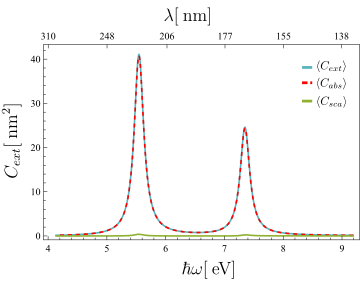
\includegraphics[width=.445\textwidth]{../../Figuras/AlContribuciones3.pdf} \label{Contribuciones}}\quad%
	\sidesubfloat[]{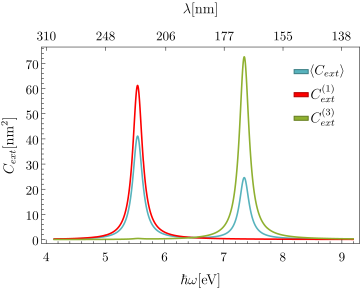
\includegraphics[width=.44\textwidth]{../../Figuras/CextAlbueno.pdf}\label{Cextpromedio}}%
	\caption{Secciones transversales como función de la energía $\hbar\omega$ y de la longitud de onda $\lambda$ para una partícula elipsoidal oblata de aluminio caracterizada por su función dieléctrica dada por el modelo de Drude ($\hbar\omega_p=13.142\text{ eV}$, $\hbar\gamma=0.197\text{ eV}$), con semiejes $a=b=1.5\text{ nm}$, $c=1\text{ nm}$ e inmersa en un medio acuoso ($n_m=1.33$). \textbf{a)}  Sección transversal de extinción promedio $\langle C_{ext}\rangle$ , sección transversal de absorción promedio $\langle C_{abs}\rangle$ y sección transversal de esparcimiento promedio $\langle C_{sca}\rangle$ en escala logarítmica. \textbf{b)} Sección transversal de extinción promedio $\langle C_{ext}\rangle$, sección transversal de extinción al iluminar a la partícula con una onda polarizada en la dirección $\hat{e}_x$ $C_{ext}^{(1)}$  y sección transversal de extinción al iluminar la partícula con una onda polarizada en la dirección $\hat{e}_z$ $C_{ext}^{(3)}$.} \label{fig:test}
\end{figure}

\noindent A partir de los resultados de la Fig. \ref{Contribuciones}, se observa que en partículas en el regimen cuasiestático, la absorción tiene una contribución mayor en la extinción que el esparcimiento. En consecuencia de lo anterior, en los resultados siguientes se analizan únicamente las secciones transversales de extinción. \\


 Para estudiar la diferencia entre considerar la sección transversal promedio y las correspondientes a iluminar la partícula con una onda polarizada en una sola dirección, en la Fig. \ref{Cextpromedio}, se muestra la sección transversal de extinción promedio $\langle C_{ext}\rangle$, la sección transversal de extinción al iluminar a partícula con una onda polarizada en la dirección $\hat{e}_x$ ($C_{ext}^{(1)}$)  y la sección transversal de extinción al iluminar la partícula con una onda polarizada en la dirección $\hat{e}_z$ ($C_{ext}^{(3)}$), para un sistema con las mismas características que el de la Fig. \ref{Contribuciones}. En esta figura se puede observar que dado que se trata de un elipsoide oblato, al considerar $\langle C_{ext}\rangle$ se observan dos frecuencias en las que la sección transversal es máxima, las cuales coinciden con las frecuencias asociadas a $C_{ext}^{(1)}$ y $C_{ext}^{(3)}$ cuando estas se maximizan. \\

A continuación se presentan los cálculos de las secciones tranversales de extinción promedio  $\langle C_{ext}\rangle$ considerando nanopartículas elipsoidales oblatas cuya función dieléctrica está caracterizada por el modelo de Drude para aluminio \cite{Aluminio} y por datos experimentales para plata \cite{Plata}, oro \cite{Plata}, bismuto \cite{Bismuto} y  óxido de magnesio \cite{MgO}.



\subsection*{Aluminio y plata}
En la Fig. \ref{aluminioplataAR} se muestran las secciones transversales de extinción promedio en función de la energía $\hbar\omega$ y de la longitud de onda $\lambda$ para partículas elipsoidales oblatas de aluminio [Fig. \ref{aluminioAR}] y plata [Fig. \ref{plataAR}], cuyas funciones dieléctricas están dadas por el modelo de Drude con parámetros $\hbar\omega_p=13.142\text{ eV}$, $\hbar\gamma=0.197\text{ eV}$ y datos experimentales obtenidos de \cite{Plata}, respectivamente. Las partículas están inmersas en un medio acuoso ($n_m=1.33$) y  presentan relaciones de aspecto AR$=2$, con excepción de la línea gris punteada, que corresponde al caso de una esfera para la cual AR$=1$. 
\begin{figure}[h!]
	\sidesubfloat[]{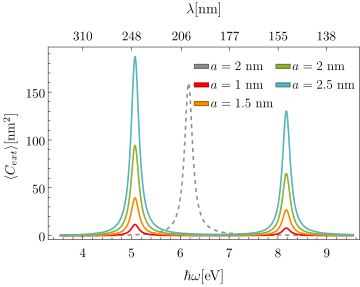
\includegraphics[width=.445\textwidth]{../../Figuras/AlAR} \label{aluminioAR}}\quad%
	\sidesubfloat[]{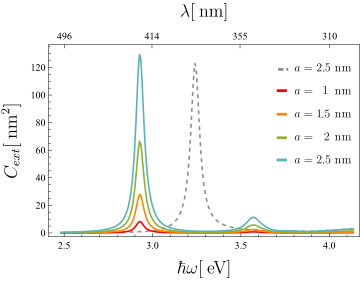
\includegraphics[width=.44\textwidth]{../../Figuras/AgAR}\label{plataAR}}%
	\caption{Secciones transversales de extinción promedio $\langle C_{ext}\rangle$ como función de la energía $\hbar\omega$ y de la longitud de onda $\lambda$ para una partícula elipsoidal oblata con razón de aspecto $AR=a/c=2$ constante, excepto en el caso de una esfera (línea gris punteada) donde $AR=1$, e inmersa en un medio acuoso ($n_m=1.33$). La partícula está caracterizada por su función dieléctrica dada por  \textbf{a)} el modelo de Drude para el aluminio ($\hbar\omega_p=13.142\text{ eV}$, $\hbar\gamma=0.197\text{ eV}$) y \textbf{b)} datos experimentales correspondientes a la plata obtenidos de \cite{Plata}. }\label{aluminioplataAR}
\end{figure}\\

\noindent De los resultados de la Fig. \ref{aluminioplataAR}, se observan dos máximos locales correspondientes a las frecuencias a las cuales $\langle C_{ext}\rangle$ se maximiza al iluminar la partícula en la dirección $\hat{e}_x$ a 254 nm para aluminio y 434 nm para plata y en la dirección $\hat{e}_z$
a 146 nm para aluminio y 344 nm para la plata. Como las transiciones interbanda de la plata y el aluminio ocurren a , estas resonancias se atribuyen a resonancias plasmónicas

La absorción en el aluminio es fuerte en el UV, lo que permite modos plasmónicos bien separados.


 En las Figs. \ref{aluminioc}  y \ref{platac} se observan las secciones transversales de extinción promedio para partículas de aluminio y plata, respectivamente, con una relación de aspecto variable; se observa que conforme la relación de aspecto se aproxima a la unidad, hay un corrimiento de las frecuencias asociadas a las $\langle C_{ext}\rangle$ máximas hacia la frecuencia de resonancia (aluminio: $201\text{ nm}$, plata: $383\text{ nm}$) asociada a una esfera  inmersa en agua. Tanto en el caso del aluminio como el de la plata se observa que al aumentar su relación de aspecto, así como la longitud de su eje mayor, la $\langle C_{ext}\rangle$ aumenta.



\begin{figure}[h!]
	\sidesubfloat[]{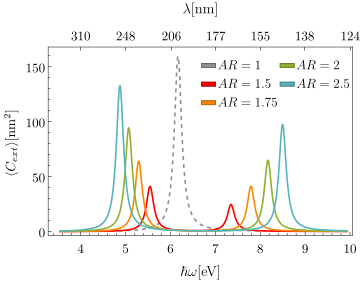
\includegraphics[width=.445\textwidth]{../../Figuras/Alc} \label{aluminioc}}\quad%
	\sidesubfloat[]{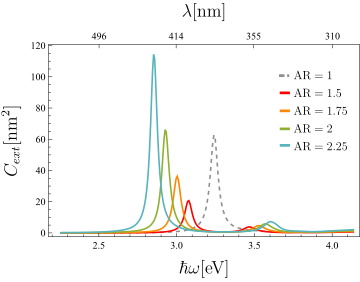
\includegraphics[width=.44\textwidth]{../../Figuras/Agc}\label{platac}}%
	\caption{Secciones transversales de extinción promedio $\langle C_{ext}\rangle$ como función de la energía $\hbar\omega$ y de la longitud de onda $\lambda$ para una partícula elipsoidal oblata con razón de aspecto con semieje menor $c=1nm$ constante, e inmersa en un medio acuoso ($n_m=1.33$). La partícula está caracterizada por su función dieléctrica dada por  \textbf{a)} el modelo de Drude para el aluminio ($\hbar\omega_p=13.142\text{ eV}$, $\hbar\gamma=0.197\text{ eV}$) y \textbf{b)} datos experimentales correspondientes a la plata obtenidos de \cite{Plata}.}\label{aluminioplatac}
\end{figure}

\subsection*{Oro y bismuto}
En la Fig. \ref{oro} se observan las secciones transversales de extinción promedio para partículas de oro, así como la parte imaginaria y real de su función dieléctrica. En la Fig. \ref{oroAR} se consideraron partículas con relación de aspecto AR$=2$ y en la Fig. \ref{oroc} se consideraron partículas con relación de aspecto variable; se observa que conforme la relación de aspecto se aproxima a la unidad, hay un corrimiento de las frecuencias asociadas a las $\langle C_{ext}\rangle$ máximas hacia una frecuencia de resonancia ($557\text{ nm}$) asociada a una esfera de oro inmersa en agua. 


La absorción en el oro es fuerte en el visible, lo que suprime resonancias adicionales


\begin{figure}[H]
	\sidesubfloat[]{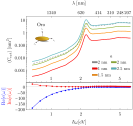
\includegraphics[width=.445\textwidth]{../../Figuras/Au2} \label{oroAR}}\quad%
	\sidesubfloat[]{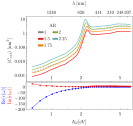
\includegraphics[width=.44\textwidth]{../../Figuras/Au}\label{oroc}}%
	\caption{Secciones transversales de extinción promedio $\langle C_{ext}\rangle$ como función de la energía $\hbar\omega$ y de la longitud de onda $\lambda$ para una partícula elipsoidal oblata de oro, cuyo índice de refracción complejo fue obtenido a partir de datos experimentales  e inmersa en agua ($n_m=1.33$) y curvas de comparación del índice de refracción (parte real en azul, parte imaginaria en rojo) como función de la energía $\hbar\omega$ y de la longitud de onda $\lambda$ para el oro. \textbf{a)} Razón de aspecto $AR=2$ constante, excepto en el caso de una esfera (línea gris punteada) donde $AR=1$. \textbf{b)} Semieje menor $c=1$ nm constante.}\label{oro}
\end{figure}


En la Fig. \ref{bismuto} se observan las secciones transversales de extinción promedio para partículas de bismuto, así como la parte imaginaria y real de su índice de refracción. En la Fig. \ref{bismutoAR} se consideraron partículas con relación de aspecto AR$=2$  y en la Fig. \ref{bismutoc} se consideraron partículas con relación de aspecto variable. En ambas figuras es posible observar una frecuencia de resonancia de alrededor de los 154 nm.

\begin{figure}[H]
	\sidesubfloat[]{\includegraphics[width=.445\textwidth]{../../Figuras/Bi2} \label{bismutoAR}}\quad%
	\sidesubfloat[]{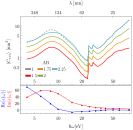
\includegraphics[width=.44\textwidth]{../../Figuras/Bi}\label{bismutoc}}%
	\caption{Secciones transversales de extinción promedio $\langle C_{ext}\rangle$ como función de la energía $\hbar\omega$ y de la longitud de onda $\lambda$ para una partícula elipsoidal oblata de bismuto, cuyo índice de refracción complejo fue obtenido a partir de datos experimentales  e inmersa en agua ($n_m=1.33$) y curvas de comparación de la función dieléctrica (parte real en azul, parte imaginaria en rojo) como función de la energía $\hbar\omega$ y de la longitud de onda $\lambda$ para el bismuto. \textbf{a)} Razón de aspecto $AR=2$ constante, excepto en el caso de una esfera (línea gris punteada) donde $AR=1$. \textbf{b)} Semieje menor $c=1$ nm constante.}\label{bismuto}
\end{figure}


\subsection*{Óxido de magnesio}
En la Fig. \ref{mgo} se observan las secciones transversales de extinción promedio para partículas de bismuto, así como la parte imaginaria y real de su índice de refracción. En la Fig. \ref{mgoAR} se consideraron partículas con relación de aspecto AR$=2$  y en la Fig. \ref{mgoc} se consideraron partículas con relación de aspecto variable. En ambos casos se observa que la $\langle C_{ext}\rangle$ tiene un comportamiento creciente pues, dado que en el espectro de las ondas de radio, la contribución de la absorción es nula y la única contribución es la del esparcimiento, que aumenta al disminuir la longitud de onda.

\begin{figure}[H]
	\sidesubfloat[]{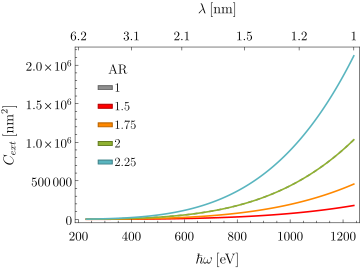
\includegraphics[width=.445\textwidth]{../../Figuras/MgOc} \label{mgoc}}\quad%
	\sidesubfloat[]{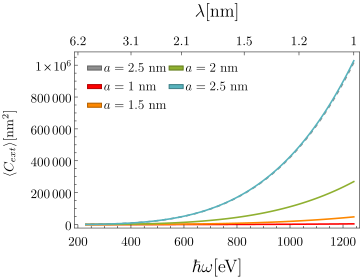
\includegraphics[width=.44\textwidth]{../../Figuras/MgOAR}\label{mgoAR}}%
	\caption{Secciones transversales de extinción promedio $\langle C_{ext}\rangle$ como función de la energía $\hbar\omega$ y de la longitud de onda $\lambda$ para una partícula elipsoidal oblata de óxido de magnesio, cuyo índice de refracción complejo fue obtenido a partir de datos experimentales  e inmersa en agua ($n_m=1.33$) y curvas de comparación de la función dieléctrica (parte real en azul, parte imaginaria en rojo) como función de la energía $\hbar\omega$ y de la longitud de onda $\lambda$ para el bismuto. \textbf{a)} Razón de aspecto $AR=2$ constante, excepto en el caso de una esfera (línea gris punteada) donde $AR=1$. \textbf{b)} Semieje menor $c=1$ nm constante.}\label{mgo}
\end{figure}

Tiene transiciones interbanda a energías muy bajas (~0.15 - 0.2 eV, en el infrarrojo medio).
Se comporta como un semimetal, con una densidad de estados electrónica muy baja en el nivel de Fermi.
En el visible y el infrarrojo cercano, su respuesta óptica es más compleja y no sigue el modelo simple de plasma.







